\documentclass[9pt,a4paper]{article}
\usepackage[left=1.6cm, right= 1.6cm, top=1.0cm, bottom=1.36cm]{geometry}
\usepackage{multicol}
\usepackage[utf8]{inputenc}
\usepackage{gensymb}
\usepackage{graphicx}
\usepackage{float}
 \usepackage{fancyvrb}
\usepackage{amssymb}
\usepackage{amsmath}
\usepackage{multirow}
\usepackage{mathtools}  
\usepackage{xfrac}  
\usepackage[italicdiff]{physics}
\usepackage[center]{caption}
\newcommand{\angstrom}{\textup{\AA}}
\usepackage{biblatex}
\addbibresource{References.bib}

\DeclareMathOperator{\taninv}{tan^{-1}}
\graphicspath{ {./images/} }
\DeclareUnicodeCharacter{2212}{-}
\setlength{\columnsep}{0.6cm}
\renewcommand\thesection{\Roman{section}}
\renewcommand\thesubsection{\thesection.\Roman{subsection}}

\begin{document}
\font\myfont=cmr12 at 19pt
\title{ { \textbf{ \myfont Emission spectra of metals and Absorption spectrum of Iodine vapour using constant deviation spectrometer }}}
\author{Deependra Singh}
\date{$2011058$}
\maketitle 
 \vspace*{0.5cm} 
\section{Abstract} 
By the quantam description of energy states, the emission spectra of metals is due to excitation and de-excitation of electrons through the various discrete energy levels of their bound states. As the electrons de-excite they emit light of energy corresponding to the energy gap. Since a spectrum is unique to a element, it is used for its detection. By using a constant deviation prism, which deviates the dispersed light beams at a minimum deviation of $90 \degree$, we can observe and study the different wavelength of light emitted by the source. In the experiment, we will be studying the emission spectra of metals (Brass, Cu) and absorption spectrum of iodine vapours.


\vspace*{0.5cm}
\begin{multicols*}{2}
\noindent

\section{Theory}
\subsection{Constant Deviation Spectrometer}
An instrument used to study the spectra with unaided eye is called spectroscope or spectrometer. For this experiment a constant deviation prism of angle of minimum deviation $90 \degree$ is used such that the emission spectrum can be observed from a telescope placed perpendicular to the source and collimator (incident beam). For this purpose, the prism is comprised of three parts: two $30 \degree$ prisms, PQR and QST along with the reflecting prism PRS as shown in figure below. When the angle of incidence is equal to the angle of emergence and the
angle of deviation is $90 \degree$, a ray would be passing through a position of minimum deviation. 

\begin{figure}[H]
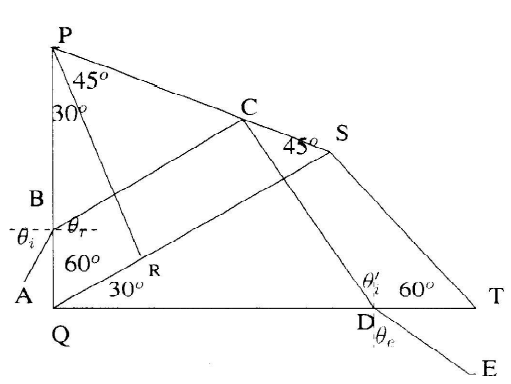
\includegraphics[height=3.5cm, width=6cm]{MP2.png}
\caption{\textbf{Constant deviation Prism}}
\label{fig1}
\end{figure}

\subsection{Emission spectra of metals}
Two observe the absorption spectra of the metals, the prism firstly needs to be calibrated. For this purpose a mercury lamp of known wavelength and spectrum is used as a source. The experimental setup consists of the source, a collimator and the constant deviation prism. A telescope placed perpendicular to the collimator to observe the spectra as shown in figure below. A calibrated cylinder which is to be rotated till the adjust the prism until the angle of minimum deviation is obtained for a wavelength, which could then be observed from the prism. For the calibration part, the prism will be adjusted to almost match the wavelgth on the cylinder for a beam observed with the given value. Then the observed wavelength in spectra will be plotted against the given wavelengths to obtain a calibration parameter for further data. For the spectra of metals, the metal source will be heated and placed in front of the collimator. The heating will excite the electrons and the further de excitation will produce the emission spectra.


\begin{figure}[H]
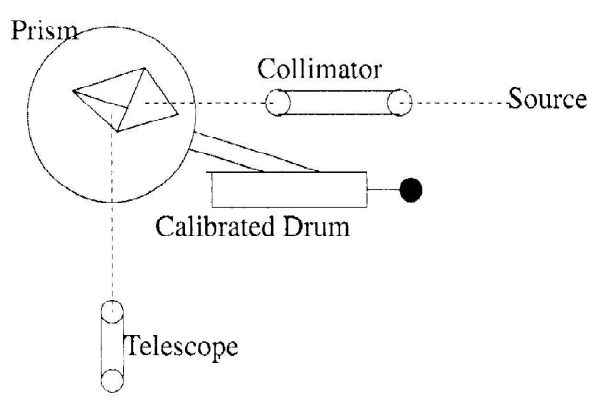
\includegraphics[height=4cm, width=7cm]{MP3.png}
\caption{\textbf{Experimental Setup}}
\label{fig2}
\end{figure}

\subsection{Absorption Spectrum of Iodine Vapour}
Iodine absorption spectrum can be explained by vibronic tranisitions between the energy levels of different quantum states defined by their vibrational quantum numbers. For this experiment Iodine vapours are excited by a source of white light and missing (absorbed) wavelengths of light  are observed in the spectrum which appear as dark bands. The absorption involves the following transition: $(X, \nu'') \rightarrow (B, \nu')$\\
where X represents the ground state and B is the first excited electronic energy state. $\nu'' (=0, 1, 2\; etc)$ and $\nu' (=0,1,2,\; etc)$ represent the vibrational quantum numbers in the ground and excited electronic states, respectively.\\\\
As shown in the figure, for transitions between the ground state and first excited state at room temperature, the first transition corresponds to $\nu'' =0$ to $\nu' = 0$ which is labelled as $0\leftarrow0$ absorption line.\\

\begin{figure}[H]
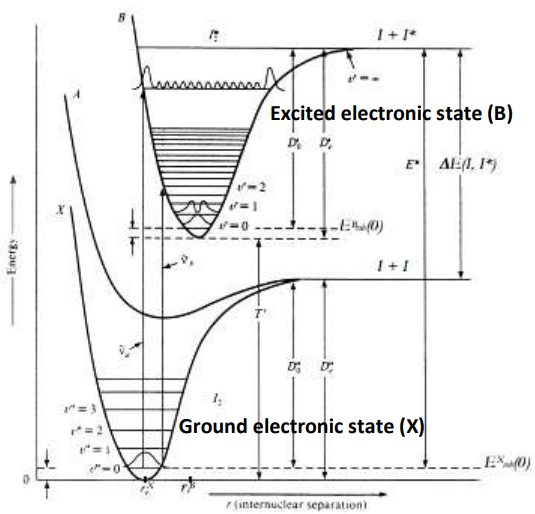
\includegraphics[height=8cm, width=8cm]{MP4.png}
\caption{\textbf{Schematic energy level diagram of iodine}}
\label{fig3}
\end{figure}

According to Franck-Condon principle, only those wavefunctions of the two stat don't significantly overlap with the ground state wavefunction, therefore usually the transition from $20\;to\;50\leftarrow0$ takes place. For the maximum energy level $\nu_{max}$ the energies form a continuum rather than being quantized and hence bond dissociation occurs given by:
\[(D_0)=\;E(\nu'=\nu_{max})-E(\nu'=0)\]

Since the vibronix energy levels are coarsely placed, one can apply the simple harmonic oscillator equations involving Morse potential ro solve for energy levels, giving the force constant to be: 
\[f=4\pi^2 \mu(\Delta\bar{\nu_{e^{avg}}})\]




\vspace*{0.2cm}
\section{Observation and Table}
Least Count of Calibrated Drum= $10\;\AA$\\\\
\textbf{Table for calibration using mercury lamp:}
\begin{table}[H]
\centering
\resizebox{6cm}{2.5cm}{ \begin{tabular}{||c|c|c||}
\hline
 & &  \\
Sl. No &  $\lambda_{given}$   &  $\lambda_{observed}$ \\
         &($\AA$) & ($\AA$)  \\ \hline
1	&	5770	&	5870	\\ \hline
2	&	5790	&	5890	\\ \hline
3	&	5461	&	5550	\\ \hline
4	&	6152	&	6060	\\ \hline
5	&	6234	&	6300	\\ \hline
6	&	5025	&	4970	\\ \hline
7	&	4358	&	4410	\\ \hline
8	&	4078	&	4110	\\ \hline
9	&	4047	&	4080	\\ \hline
\end{tabular}  
}\caption{\label{tab1}\textbf{For calibration using mercury lamp}} 
\end{table}

\begin{figure}[H]
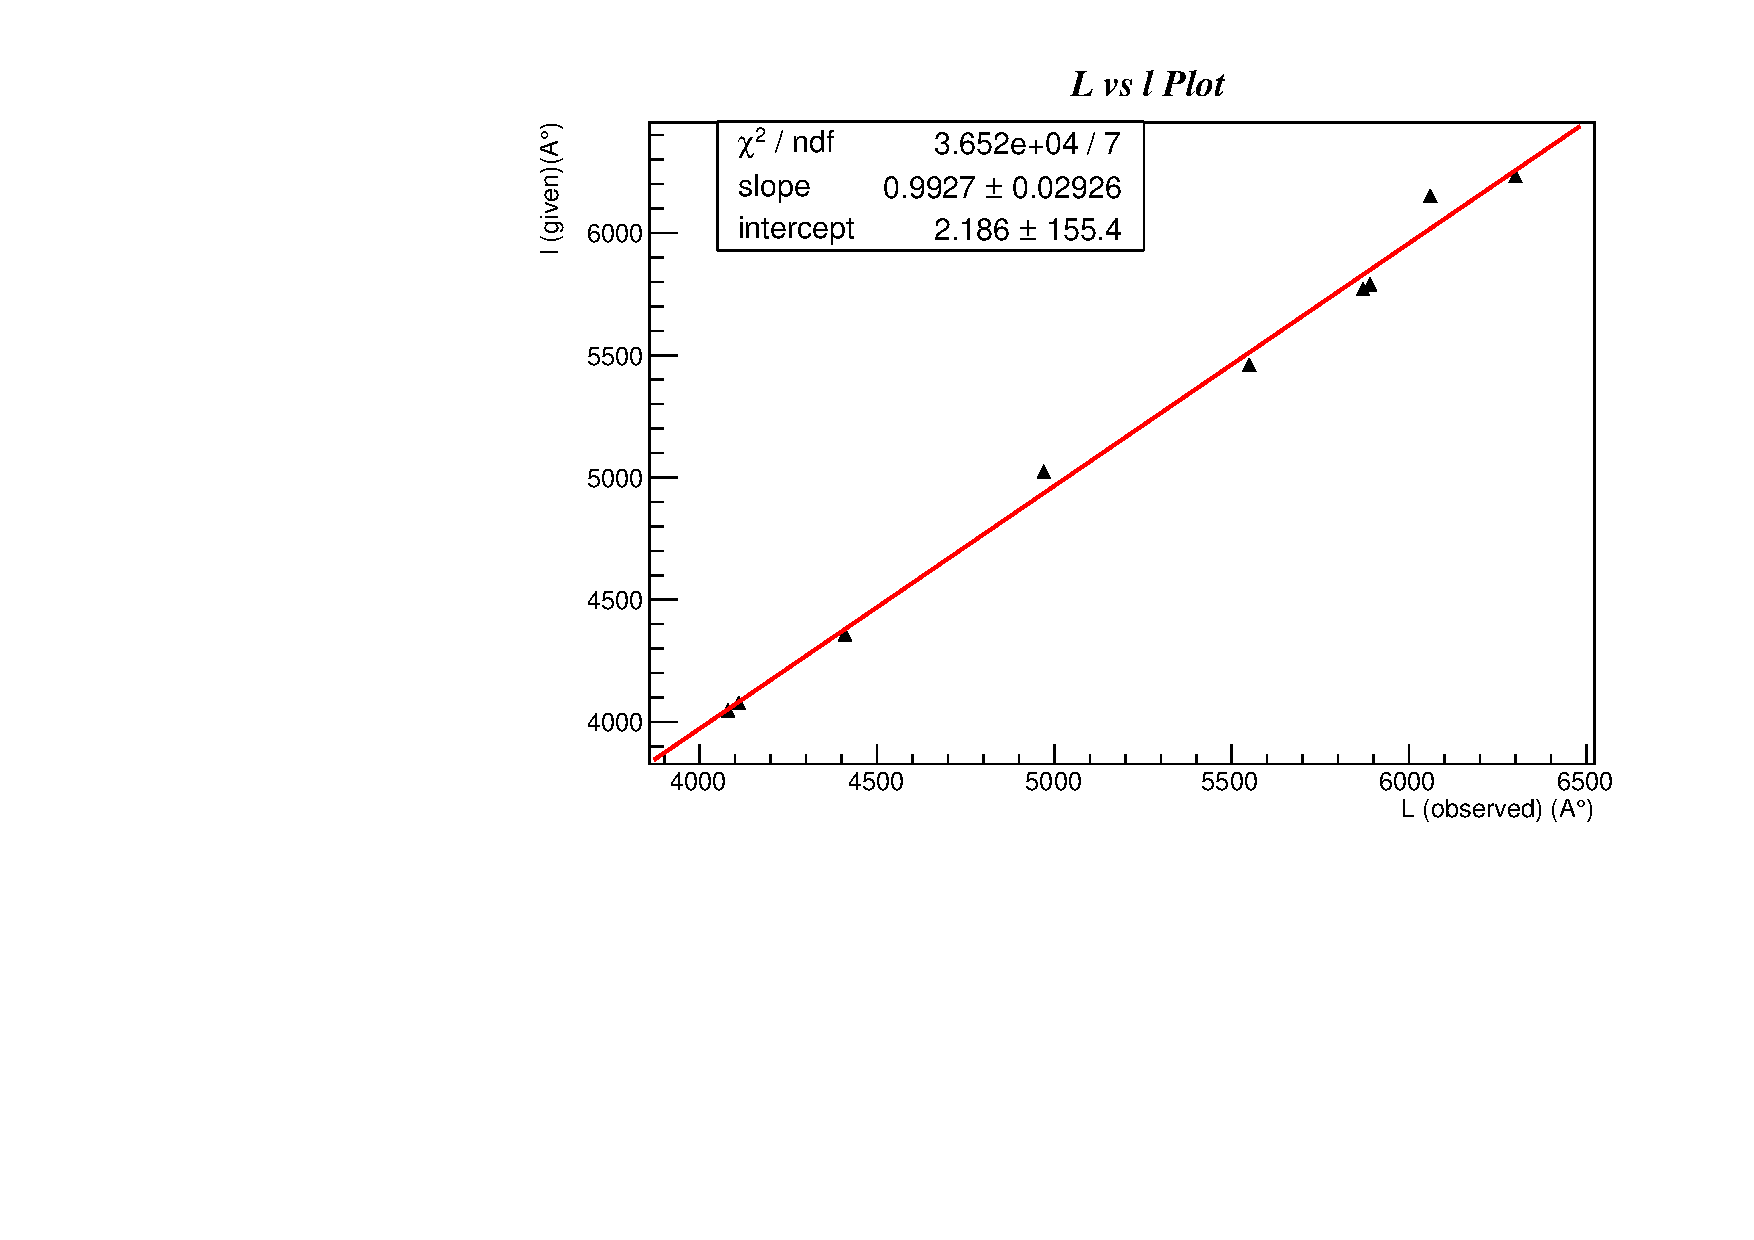
\includegraphics[height=7cm, width=9.4cm]{MP1}
\caption{\textbf{$\lambda_{given}(l)\;vs\;\lambda_{observed} (L)$ Plot}}
\label{fig4}
\end{figure}

Calibration Parameter= slope $(m)=0.9927$\\\\
{}$\lambda_{corrected}=m\lambda_{observed}$\\\\

\textbf{Table for emission spectrum of metals:}
\begin{itemize}
\item \textbf{For Brass:}
\begin{table}[H]
\centering
\resizebox{6.5cm}{3cm}{ \begin{tabular}{||c|c|c|c||}
\hline
 & & &  \\
Sl. No &  $\lambda_{observed}$   &  $\lambda_{corrected}$ &$\lambda_{lit}$ \\
         &($\AA$) & ($\AA$)  & ($\AA$) \\ \hline
1	&	6490	&	6484	&	6484.4	\\ \hline
2	&	6010	&	6004	&	6013.4 	\\ \hline
3	&	5880	&	5874	&	5890.4 	\\ \hline
4	&	5790	&	5784	&	5842.5	\\ \hline
5	&	5380	&	5375	&	5375.3	\\ \hline
6	&	5310	&	5305	&	5308.6	\\ \hline
7	&	5240	&	5235	&	5234.5 	\\ \hline
8	&	5180	&	5175	&	5176.0	\\ \hline
9	&	4870	&	4865	&	4866.3 	\\ \hline
10	&	4780	&	4775	&	4773.0	\\ \hline
11	&	4740	&	4735	&	4738.0	\\ \hline
12	&	4580	&	4575	&	4575.0	\\ \hline
13	&	4540	&	4535	&	4533.8	\\ \hline
14	&	4440	&	4436	&	4435.7	\\ \hline
15	&	4320	&	4316	&	4308.7 	\\ \hline
16	&	4100	&	4096	&	4089.5	\\ \hline

\end{tabular}  
}\caption{\label{tab2}\textbf{Emission Spectrum for Brass}} 
\end{table}

\item \textbf{For Copper:}
\begin{table}[H]
\centering
\resizebox{6.5cm}{2.9cm}{ \begin{tabular}{||c|c|c|c||}
\hline
 & & &  \\
Sl. No &  $\lambda_{observed}$   &  $\lambda_{corrected}$ &$\lambda_{lit}$ \\
         &($\AA$) & ($\AA$)  & ($\AA$) \\ \hline
1	&	6480	&	6474	&	6475.4	\\ \hline
2	&	5880	&	5874	&	5890.4	\\ \hline
3	&	5790	&	5784	&	5783.9 	\\ \hline
4	&	5370	&	5365	&	5365.5	\\ \hline
5	&	5300	&	5295	&	5297.4 	\\ \hline
6	&	5220	&	5215	&	5207.3 	\\ \hline
7	&	5190	&	5185	&	5184.1 	\\ \hline
8	&	4870	&	4865	&	4866.3	\\ \hline
9	&	4770	&	4765	&	4766	\\ \hline
10	&	4760	&	4755	&	4753.5 	\\ \hline
11	&	4710	&	4705	&	4702.1	\\ \hline
12	&	4550	&	4545	&	4546.4	\\ \hline
13	&	4430	&	4426	&	     4422.5 	\\ \hline
14	&	4320	&	4316	&	     4308.7 	\\ \hline
15	&	4110	&	4106	&	4104.2	\\ \hline

\end{tabular}  
}\caption{\label{tab3}\textbf{Emission Spectrum for Copper}} 
\end{table}
\end{itemize}
\vspace*{0.5cm}
\textbf{Table for absorption spectrum of iodine:}

\begin{table}[H]
\centering
\resizebox{8cm}{4.5cm}{ \begin{tabular}{||c|c|c|c|c||}
\hline
 & & & & \\
Sl. No &  $\lambda_{observed}$   &  $\lambda_{corrected}$ & Wave Number\;$\bar{\nu_e}$ & Difference in wave number  \\
         &($\AA$)  & ($\AA$) & $(cm^{-1})$ &  $\Delta\bar{\nu_e} (cm^{-1})$\\ \hline

1	&	6360	&	6354	&	15738.12	&	432.64	\\ \hline
2	&	6190	&	6184	&	16170.76	&	105.28	\\ \hline
3	&	6150	&	6144	&	16276.04	&	79.86	\\ \hline
4	&	6120	&	6114	&	16355.9	&	134.87	\\ \hline
5	&	6070	&	6064	&	16490.77	&	109.5	\\ \hline
6	&	6030	&	6024	&	16600.27	&	83.08	\\ \hline
7	&	6000	&	5994	&	16683.35	&	140.34	\\ \hline
8	&	5950	&	5944	&	16823.69	&	142.72	\\ \hline
9	&	5900	&	5894	&	16966.41	&	86.8	\\ \hline
10	&	5870	&	5864	&	17053.21	&	87.69	\\ \hline
11	&	5840	&	5834	&	17140.9	&	88.6	\\ \hline
12	&	5810	&	5804	&	17229.5	&	89.52	\\ \hline
13	&	5780	&	5774	&	17319.02	&	120.81	\\ \hline
14	&	5740	&	5734	&	17439.83	&	91.73	\\ \hline
15	&	5710	&	5704	&	17531.56	&	61.68	\\ \hline
16	&	5690	&	5684	&	17593.24	&	124.69	\\ \hline
17	&	5650	&	5644	&	17717.93	&	63.01	\\ \hline
18	&	5630	&	5624	&	17780.94	&	63.46	\\ \hline
19	&	5610	&	5604	&	17844.4	&	96.04	\\ \hline
20	&	5580	&	5574	&	17940.44	&	97.08	\\ \hline
21	&	5550	&	5544	&	18037.52	&	131.08	\\ \hline
22	&	5510	&	5504	&	18168.6	&	62.94	\\ \hline
23	&	5490	&	5485	&	18231.54	&	66.72	\\ \hline
24	&	5470	&	5465	&	18298.26	&	67.21	\\ \hline
25	&	5450	&	5445	&	18365.47	&	67.71	\\ \hline
26	&	5430	&	5425	&	18433.18	&	68.21	\\ \hline
27	&	5410	&	5405	&	18501.39	&	68.71	\\ \hline
28	&	5390	&	5385	&	18570.1	&	69.23	\\ \hline
29	&	5370	&	5365	&	18639.33	&	69.74	\\ \hline
30	&	5350	&	5345	&	18709.07	&	70.27	\\ \hline
31	&	5330	&	5325	&	18779.34	&	106.4	\\ \hline
32	&	5300	&	5295	&	18885.74	&		\\ \hline

\end{tabular}  
}\caption{\label{tab4}\textbf{Absorption Spectrum for Iodine}} 
\end{table}
\vspace*{0.5cm}
\section{Calculation}

Bond Dissociation Energy $(D_0)=\;E(\nu'=\nu_{max})-E(\nu'=0)$\\
\[E(\nu'=\nu_{max})=hc\nu_{max}\]
\[\therefore\;E(\nu'=\nu_{max})=\frac{18885.74}{8068}\;eV\]
\[E(\nu_{max})=2.34\;eV\]
Similarly for lowest energy state $E(\nu'=0)$:\\
\[E(\nu'=0)=hc\nu_{min}=\frac{15738.12}{8068}\;eV\]
\[E(\nu_{min})=1.95\;eV\]
Therefore $D_0=0.39\;eV/molecule$\\\\

Force Constant is given by: $f=4\pi^2 \mu(\Delta\bar{\nu_{e^{avg}}})$\\\\
From table $\ref{tab4},\;\Delta\bar{\nu_{e^{avg}}}=101.54\;cm^{-1}$\\\\
Reduced mass $\mu= 1.05\; \cross\; 10^{−25}\; kg $\\
\[\therefore\;f=38.47\;N m^{-1}\]

\subsection{Error Analysis}

\[\delta D_0= \delta E(\nu'=\nu_{max}) + \delta E(\nu'=0)\]
\[\therefore \delta D_0= \frac{\delta\bar{\nu_{max}}}{\bar{\nu_{max}}}+\frac{\delta\bar{\nu_{min}}}{\bar{\nu_{min}}}\]
\[\delta D_0=1.16\cross10^{-6}\;eV/molecule\]

\[\delta f = \sqrt{2} f\frac{\delta (\Delta\bar{\nu_e})}{\Delta\bar{\nu_e} }\]
\[\therefore \delta f=0.005\;N m^{-1}\]
\vspace*{0.5cm}
\section{Result}
\begin{itemize}
\item $D_0=\;0.39\pm1.16\cross10^{-6}\;eV/molecule$
\item $f=38.47\pm0.005\;N m^{-1}$
\end{itemize}

\subsection{Conclusions}
\begin{itemize}
\item For the emission spectra of metals, comparing the literature value of the wavelengths with the observed wavelength, we find that they are quite close. For Brass, we find that only 2 of the observed lines are closer to that of Zn while the rest correspond to that of Cu indicating a greater percentage of Cu in brass than Zn.
\item For the absorption spectra of Iodine, the value of $f$ is close to the literature value of $41\; N m^{-1}$ while $D_0$ is far from literature value of $1.54\;eV/molecule$. The error in bond dissociation energy can be associated with the fact that during the experiment the lines green weren't visible and the 	intensity continued to decrease, thereby lowering the range of observation and thus the difference of energy between the highest and lowest energy state.
\end{itemize}
\subsection{References}
\begin{itemize}
\item Bayram, S.B. and Freamat, M.V., 2015. A Spectral Analysis of Laser Induced Fluorescence of Iodine. arXiv preprint arXiv:1507.02600.
\item https://physics.nist.gov/PhysRefData/ASD/lines$\_$form.html
\end{itemize}

\end{multicols*}
\end{document}